\clearpage
\section{Noise Reduction in the Spatial Domain}


\subsection{Adding Gaussian noise to the Lena image}
\begin{figure}[ht]
\centering
	\subfigure[Original image]{
	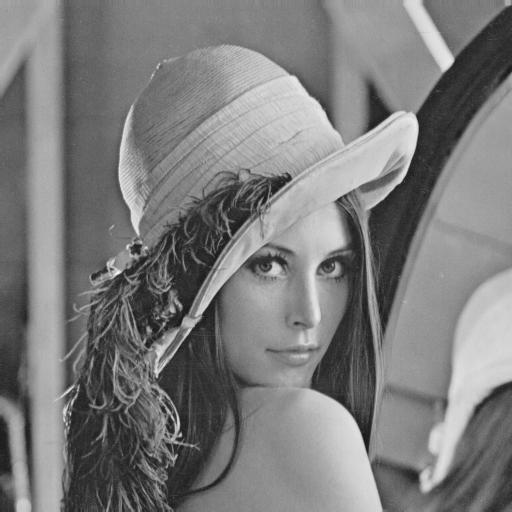
\includegraphics[width=0.45\linewidth]{question3/0_lenaBase}
	}
	\subfigure[Histogram]{
	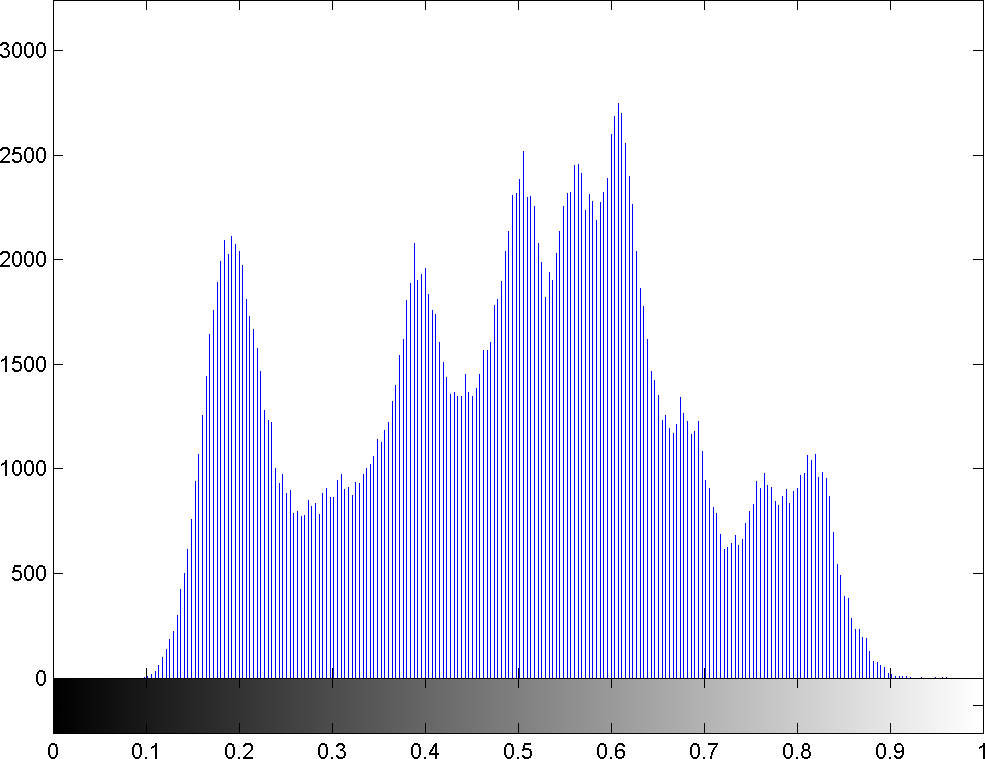
\includegraphics[width=0.45\linewidth]{question3/0_lenaBase_hist}
	}
	\subfigure[Image with Gaussian noise $\mu$=0, $\sigma^2$=0.002; PSNR +26.99dB]{
	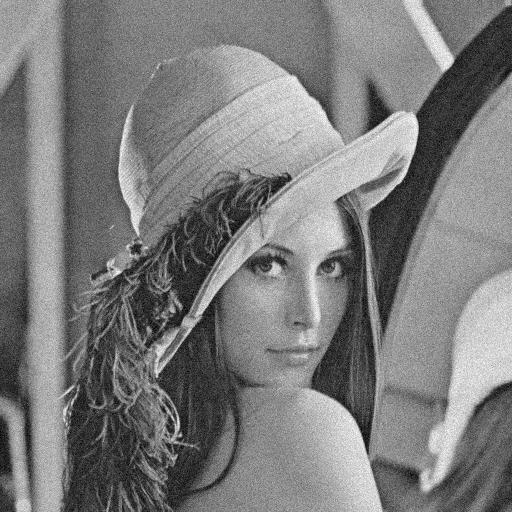
\includegraphics[width=0.45\linewidth]{question3/0_lenaNoisyGauss}
	}
	\subfigure[Histogram]{
	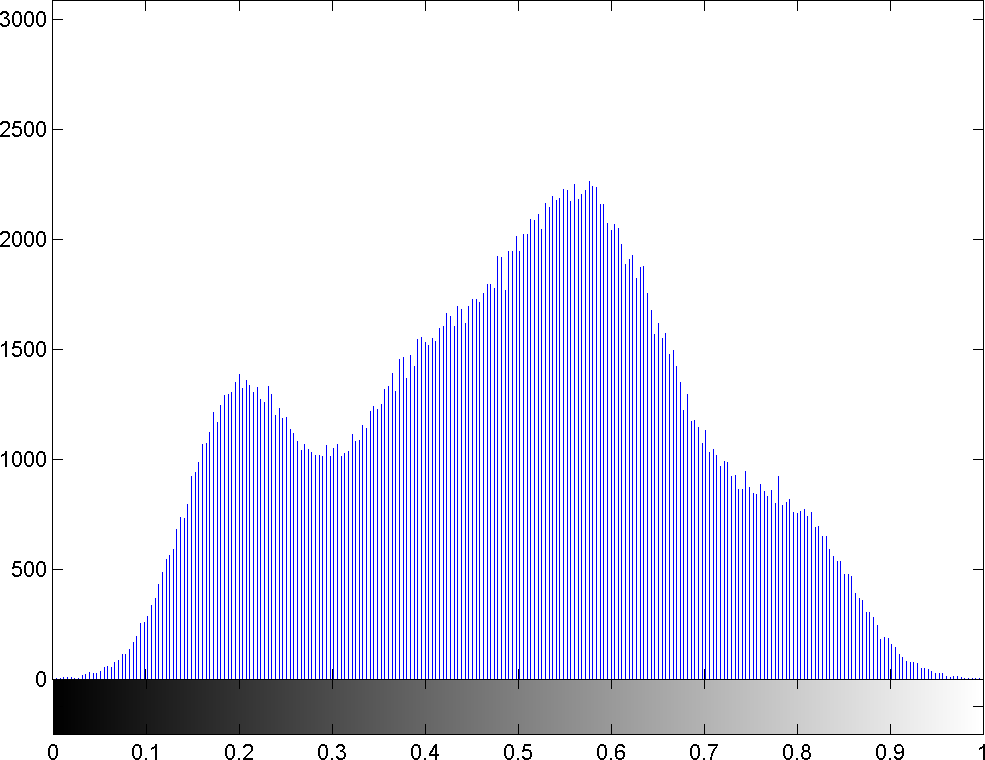
\includegraphics[width=0.45\linewidth]{question3/0_lenaNoisyGauss_hist}
	}
	\caption{Image with Gaussian noise}
\end{figure}


\clearpage
\subsection{Denoising the Lena image with a 3$\times$3 averaging kernel}
\begin{figure}[ht]
\centering
	\subfigure[Denoised image with 3$\times$3 average kernel; PSNR +30.63dB]{
	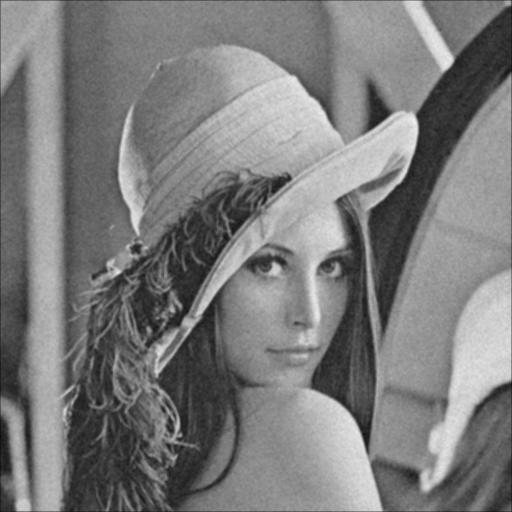
\includegraphics[width=0.45\linewidth]{question3/1_lenaDeNoisyGauss3x3avg}
	}
	\subfigure[Histogram]{
	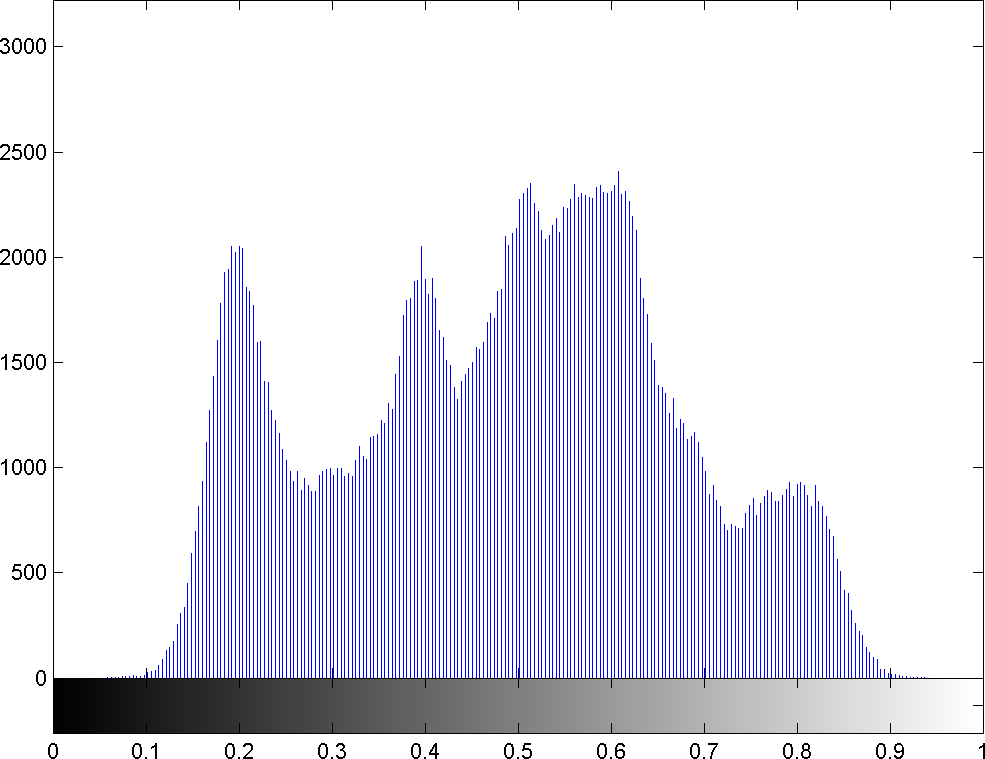
\includegraphics[width=0.45\linewidth]{question3/1_lenaDeNoisyGauss3x3avg_hist}
	}
\end{figure}

\subsubsection{Compare the visual difference between the noisy image and the denoised image. How well did it work? Why? Did the PSNR decrease?}
The denoised image appears blurrier than both the original image and the image with noise. We can assume that the denoising worked rather well as: the noise is less obvious in the denoised image, the histogram of the denoised image looks closer to the original image histogram, and the PSNR of the denoised image is higher than the noisy image.

\subsubsection{Compare the histograms of the noise-free, noisy, and denoised images. What happened? Why}
The histogram of the noisy image is missing the sharp spikes in intensities that the original image has, due to the additive nature of Gaussian noise changing each individual intensity value into a range of intensity values. The averaging filter works to partially restore these peaks by reducing the effects of Gaussian noise in a uniform area through averaging, sharpening the peak towards it's initial shape.

\subsubsection{Based on visual quality of the denoised image, what are the benefits and drawbacks associated with the average filter}
While overall noise is reduced and the PSNR of the denoised image is higher than the noisy image, perceptually, the image could be deemed worse as the image is not as sharp as the noisy image.

Averaging filters can work to reduce noise, but the stronger the averaging effect of the filter, the more edges and high frequency image details (as well as high frequency noise) are attenuated.

\clearpage
\subsection{Denoising the Lena image with a 7$\times$7 averaging kernel}
\begin{figure}[ht]
\centering
	\subfigure[Denoised image with 7$\times$7 average kernel; PSNR +26.23dB]{
	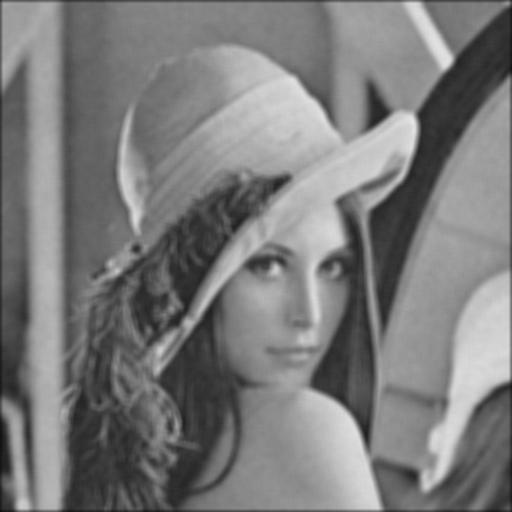
\includegraphics[width=0.45\linewidth]{question3/2_lenaDeNoisyGauss7x7avg}
	}
	\subfigure[Histogram]{
	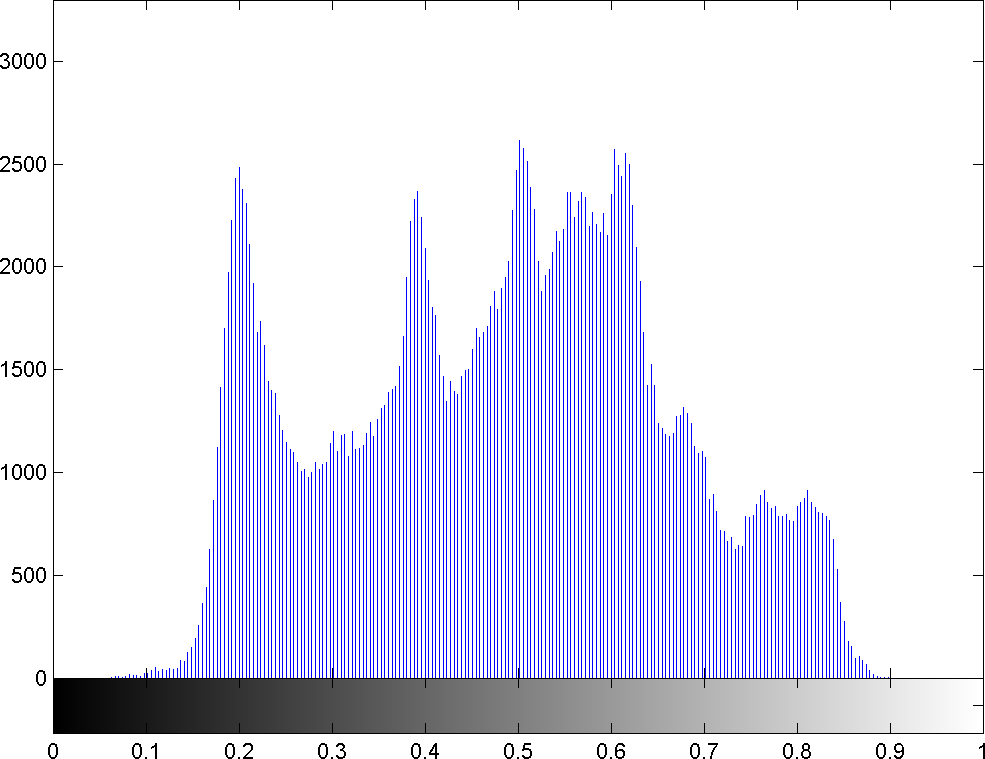
\includegraphics[width=0.45\linewidth]{question3/2_lenaDeNoisyGauss7x7avg_hist}
	}
	
	\caption{Images with Gaussian noise}
	\label{fig:gaussianNoise}
\end{figure}

\subsubsection{Compare the visual difference between the denoised image from the 7$\times$7 filtering kernel and the denoised image from the 3$\times$3 filtering kernel. Are there any differences? Why? Did the PSNR decrease? Why}

The 7$\times$7 average kernel filtered image is even blurrier than the 3$\times$3 filtered one. This is because it the kernel averages over a wider area. The PSNR of this image is also decreased, with the PSNR now slightly less than that of the noisy image. This is since the a larger the averaging window, the more high frequency details will be suppressed. While there is very little evidence of noise in the uniform areas of this image (the background), the high frequency regions such as the feathers on Lena's hat have been over-smoothed, reducing the fidelity of the image.

\subsubsection{Compare the histograms of the two denoised images. What are the differences? Why}
The histogram of the 7$\times$7 has sharper peaks than the 3$\times$3, more closely mirroring that of the original noiseless image. This is due to the large averaging window of the 7 further smoothing out extreme values in uniform areas. Therefore, what was an area of uniform intensity in the original image (and would appear as a spike in the histogram) can once again be a region of uniform intensity in the denoised image, and can regain it's peaked-ness in the histogram.


\subsubsection{Based on visual quality of the denoised image, what are the benefits and drawbacks associated with using a larger window size?}
Observing the visual quality of the 7$\times$7 kernel denoised image, the noise in the image has been highly attenuated. Uniform regions of intensity once again appear uniform.

However, the larger kernel size also highly attenuates high frequency details, therefore the sharpness of the image is highly decreased. Notably, in Lena's feathers, the once sharp contrast between feathers has been blurred, resulting in both a reduction to PSNR and perceptual visual contrast.


\clearpage
\subsection{Denoising the Lena image with a 7$\times$7 Gaussian kernel}
\begin{figure}[ht]
\centering
	\subfigure[Denoised image with 7$\times$7 Gaussian kernel; PSNR +30.82dB]{
	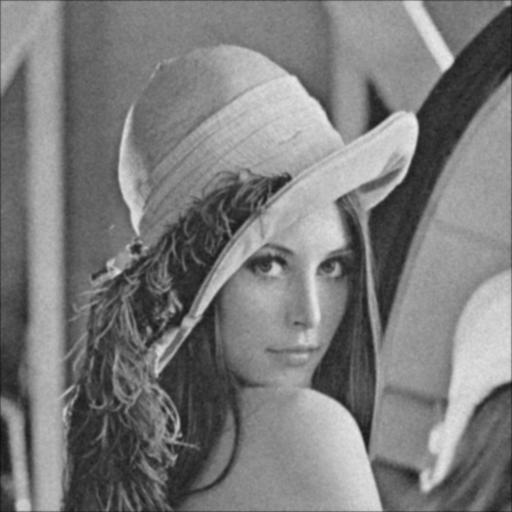
\includegraphics[width=0.45\linewidth]{question3/3_lenaDeNoisyGauss7x7avgGauss}
	}
	\subfigure[Histogram]{
	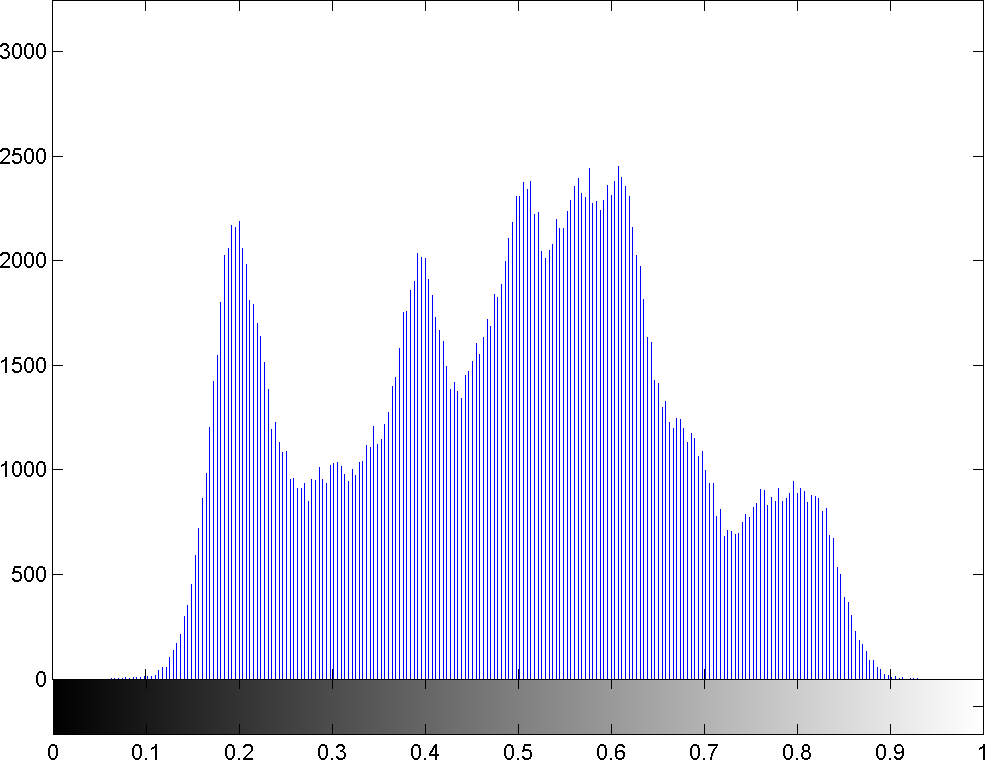
\includegraphics[width=0.45\linewidth]{question3/3_lenaDeNoisyGauss7x7avgGauss_hist}
	}
	
	\caption{Images with Gaussian noise}
	\label{fig:gaussianNoise}
\end{figure}

\subsubsection{Compare the visual difference between the denoised image from the Gaussian filtering kernel and the denoised images from the averaging filter kernels. Are there any differences? Why? Did the PSNR decrease? Why}
The Gaussian filtered image is less blurry than the two averaging filtered images. Finer details are better preserved. This is because with the Gaussian kernel, pixels further away from the centre are weighted less, unlike the uniform averaging of the averaging kernel. This weighted filtering is better at preserving edges.


\subsubsection{Compare the histograms of the denoised image using the Gaussian filtering kernel and the denoised images from the averaging filter kernels. What are the differences? Why?}
The sharp peaks seen in the 7$\times$7 averaging filter histogram are less pronounced in the Gaussian filter, as the Gaussian filter is not as good as smoothing out extreme values in uniform areas as a averaging filter. When a Gaussian kernel is centred on an extreme pixel value, the extreme value is heavily weighted, preventing the smoothing out of the extreme value.

This feature is also what allows the Gaussian filter to better preserve edge detail, so the two objectives of preserving high frequency detail and smoothing noise are in opposition.


\subsubsection{Based on visual quality of the denoised image, what are the benefits and drawbacks associated with using a Gaussian kernel as opposed to an averaging kernel?}
The Gaussian kernel results in a less blurry image than a pure averaging kernel, however does not reduce extreme values of noise as well as a pure averaging kernel.

Due to the human psycho-visual system displaying a preference for sharpness, Gaussian kernels would typically be the superior choice, irrelevant of the PSNR of the output (as PSNR does not take into account the human psycho-visual system).


\clearpage
\subsection{Denoising salt and pepper noise with blur kernels}


\subsubsection{How does the averaging filter and Gaussian filtering methods perform on the noisy image in terms of noise reduction? Explain in terms of visual quality as well as PSNR. Why do we get such results?}
Neither filter reduces the extreme noise caused by salt and pepper noise. Gaussian filtering performs much worse in term of noise reduction as extreme pixel values tend retain their original value due to the Gaussian kernel weighting. The extreme values in the pure averaging kernel are merely distributed among the neighbouring pixels, resulting in a blotch around where a pixel affected by salt and pepper noise occurred.

However, both filters result in an image that have higher PSNR than the noisy image, likely due to the extreme effect a 0 or a 1 pixel can have on the mean-{\emph squared}-error of an image. The Gaussian denoising, while not reducing the salt and pepper noise as well as the averaging filter, results in a higher PSNR as the high frequency image detail is not as highly attenuated as the straight averaging filter. 

\subsubsection{Compare the histograms of the denoised images with that of the noisy image. What characteristics are present in all of the histograms? Why?}
All the histograms of denoised images have less sharpened peaks in their histograms. The slat and pepper noise merely makes an approximately uniform reduction across the histogram and redistributes it to 0 and 1.

The blur kernels then to shift all the intensity values closer to the noisy pixels if they are included in an average, reducing the peaked-ness of the intensities in the histogram.

\begin{figure}[ht]
\centering
	\subfigure[S\&P noise on original image; PSNR +18.41dB]{
	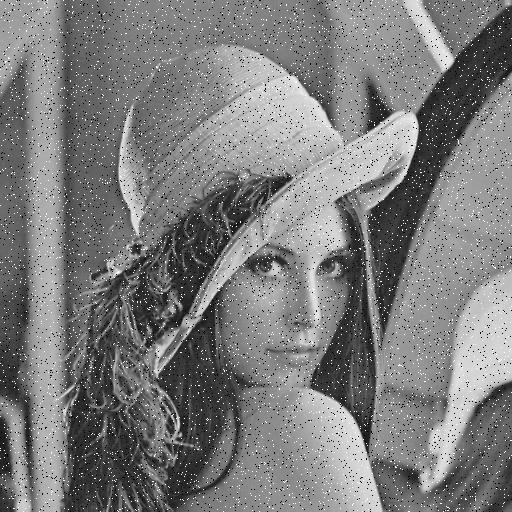
\includegraphics[width=0.45\linewidth]{question3/4_lenaNoisySp}
	}
	\subfigure[Histogram]{
	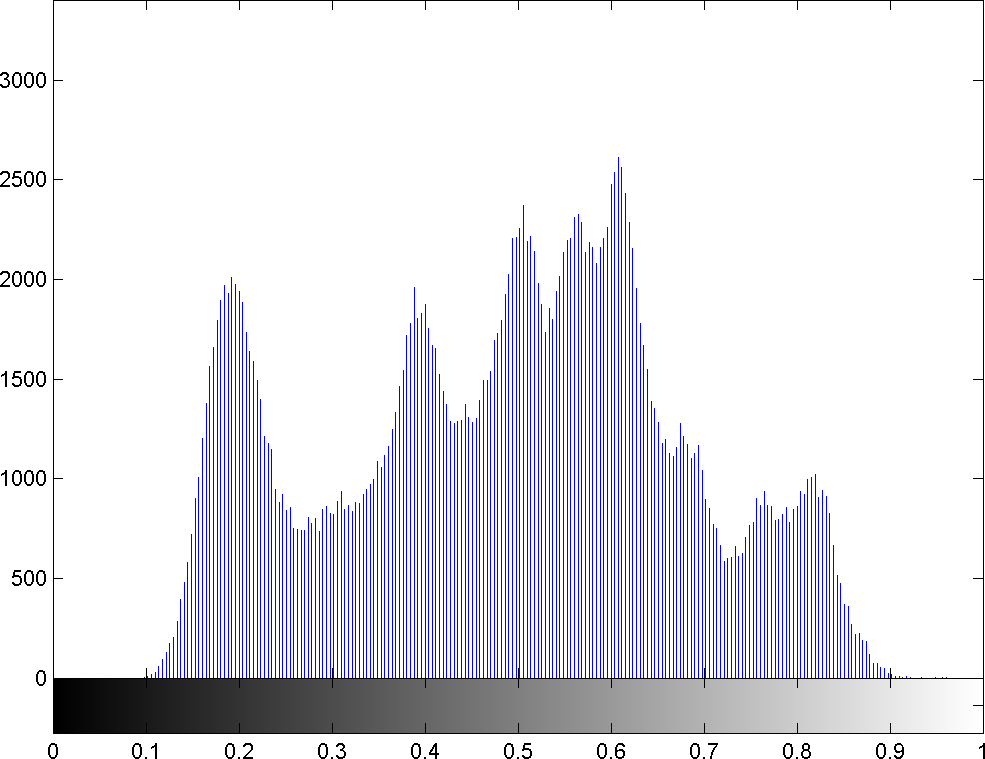
\includegraphics[width=0.45\linewidth]{question3/4_lenaNoisySp_hist}
	}
\end{figure}

\begin{figure}[ht]
\centering	
	\subfigure[S\&P denoised with 7$\times$7 average kernel; PSNR +25.52dB]{
	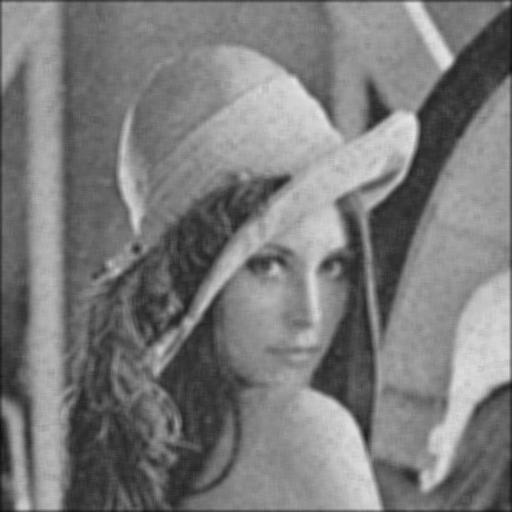
\includegraphics[width=0.45\linewidth]{question3/4_lenaDeNoisySp_7x7Avg}
	}
	\subfigure[Histogram]{
	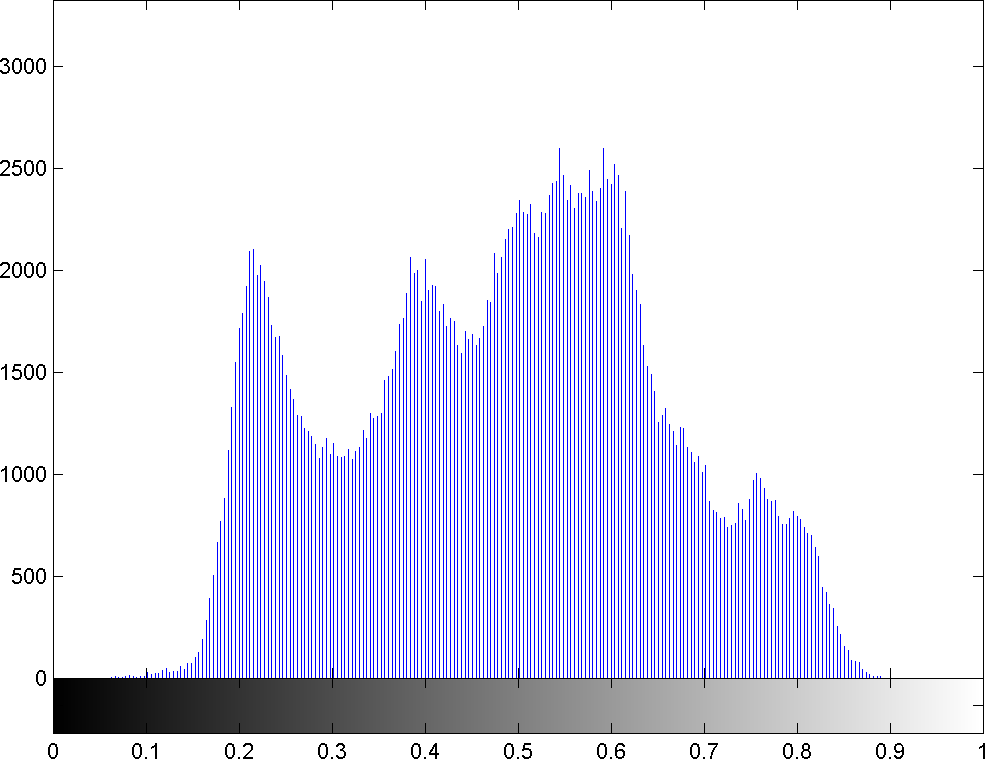
\includegraphics[width=0.45\linewidth]{question3/4_lenaDeNoisySp_7x7Avg_hist}
	}
\end{figure}

\begin{figure}[ht]
\centering
	\subfigure[S\&P denoised with 7$\times$7 Gaussian kernel; PSNR +27.08dB]{
	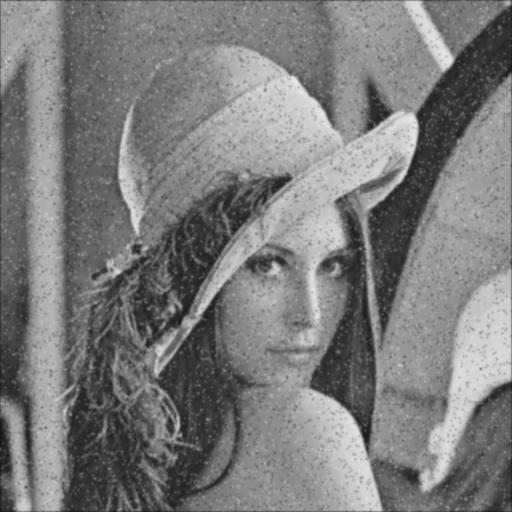
\includegraphics[width=0.45\linewidth]{question3/4_lenaDeNoisySp_7x7AvgGauss}
	}
	\subfigure[Histogram]{
	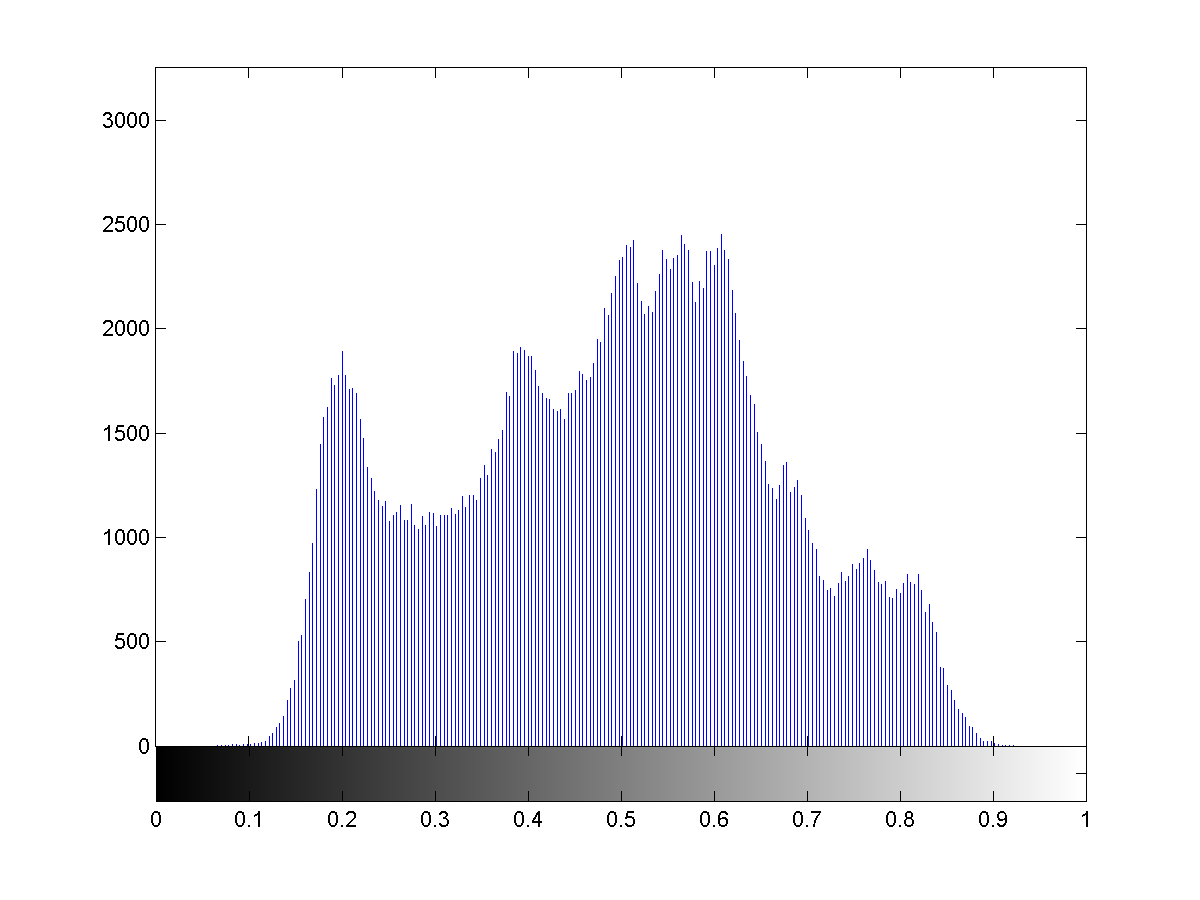
\includegraphics[width=0.45\linewidth]{question3/4_lenaDeNoisySp_7x7AvgGauss_hist}
	}
\end{figure}


\clearpage
\subsection{Denoising salt and pepper noise with a median filter}

\begin{figure}[ht]
\centering
	\subfigure[S\&P denoised with median filter; PSNR +34.47]{
	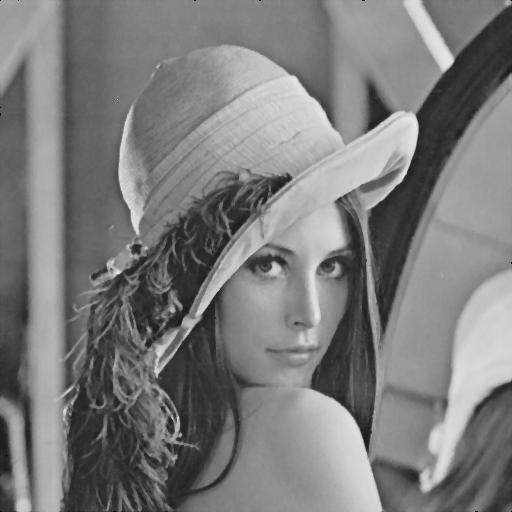
\includegraphics[width=0.45\linewidth]{question3/5_lenaDeNoisyMedian}
	}
	\subfigure[Histogram]{
	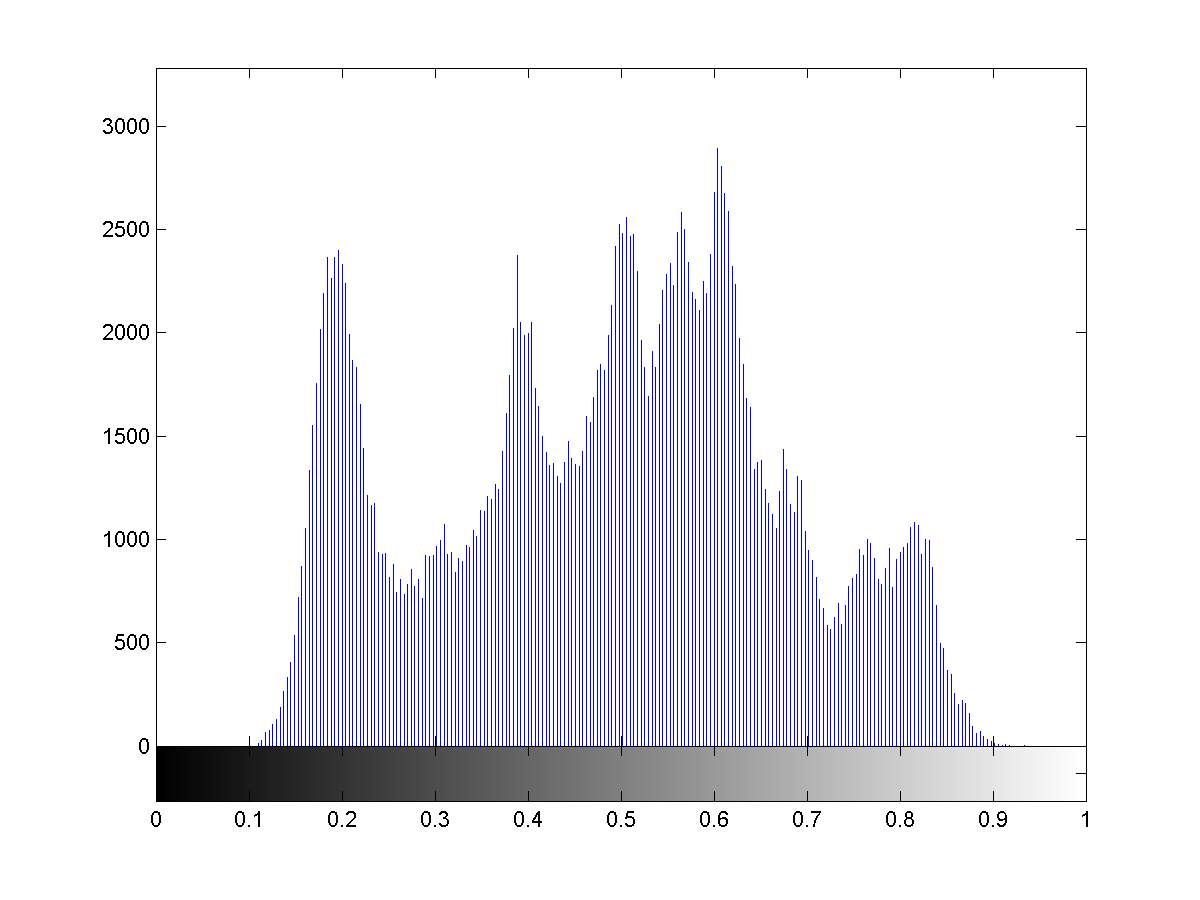
\includegraphics[width=0.45\linewidth]{question3/5_lenaDeNoisyMedian_hist}
	}
\end{figure}


\subsubsection{How does the denoised image produced using the median filter compare with the denoised images produced using averaging filter and Gaussian filtering methods? Explain in terms of visual quality as well as PSNR. Why do we get such results with median filter when compared to the other spatial filtering methods?}

The median filter produces a superior quality image compared to the Gaussian and averaging filters. The PSNR is also significantly higher.

The median filter is excellent at eliminating extreme noisy values such as salt and pepper noise as the extreme values are not taken into and average, their information is ``thrown away'' when selecting the median value from the median kernel.
